% Week 2 实验周报 v2 —— 编译方式:XeLaTeX
% v2:应导师意见,新增第 4 节"相关性与重要性分析"(图表+解读)
\documentclass[11pt]{ctexart}
\usepackage[a4paper, margin=2.5cm]{geometry}
\usepackage{booktabs}
\usepackage{graphicx}
\usepackage{hyperref}
\usepackage{enumitem}
\setlist{nosep}

\title{\textbf{Chooser Option 定价项目 —— 第 2 周实验报告(v2)}\\
\large Data Preprocessing \& Feature Engineering}
\author{佟铸城 (Zhucheng Tong)}
\date{2026 年 7 月 28 日(v2 修订:新增相关性与重要性分析)}

\begin{document}
\maketitle

\section{本周目标}
完成 Week 2 三项交付物:(1) 清洗后的结构化数据集($\geq$10 特征);(2) 自动化预处理管道(含 GitHub Actions 调度);(3) 特征工程文档。

\section{完成工作}
\begin{enumerate}
  \item \textbf{清洗管道}(\texttt{src/preprocess.py}):NYSE 交易日历对齐(以 JPM 的 1760 个交易日为主日历)、FRED 日频序列时间插值、月频 FEDFUNDS 阶梯前向填充、IQR($k=3$)离群值标记与审计;
  \item \textbf{特征工程}:共 \textbf{18 个特征}(要求 $\geq$10),分五组——多期限已实现波动率(含 Parkinson 高低价估计量)、股息(TTM 股息率、同比增速)、利率(双期限无风险利率、曲线斜率、利率动量)、市场背景(贝塔、VIX--JPM 相关性)、情绪(全部由 VIX 派生,详见第 3.4 节);
  \item \textbf{数据集输出}:全历史 1760 行;模型可用集 \textbf{1309 行、零缺失}(2019-10-17 至 2024-12-30),CSV 与 Parquet 双格式;
  \item \textbf{自动化调度}:GitHub Actions 每周五美股收盘后自动执行采集$\to$预处理$\to$提交更新,支持手动触发;研究窗口(至 2024-12-31)与实时更新窗口通过环境变量分离。
\end{enumerate}

\section{实验记录与关键发现}
\begin{enumerate}
  \item \textbf{情绪数据源变更(经导师确认)}:以 VIX 派生特征替代新闻情绪数据。任务书要求的 0--1 情绪分由 VIX 滚动 252 日百分位实现,另构造 VIX 动量与恐慌状态标记。设计上控制 VIX 的双重角色:原始水平值只作隐含波动率预期,标准化变换只作情绪状态,限制信息重叠;
  \item \textbf{离群值``标记但保留''}:被 IQR 标记的 21 个收益率极值日与 18 个 VIX 极值日经逐一核对,全部对应真实市场事件(最极端为 2020-03-13/16 COVID 崩盘)。金融数据中``离群''不等于``错误'',删除它们等于抹掉第 4 周要研究的高波动失效区间,故全部保留并留存审计文件;
  \item \textbf{与论文参数的交叉印证}:清洗后 JPM 的 21 日已实现波动率全样本均值为 26.9\%,与参考论文采用的 $\sigma = 28.2\%$ 量级一致,间接验证了数据与论文口径的可比性;
  \item \textbf{极端行情抽检}:2020-03-16 行显示单日对数收益 $-16.2\%$、VIX 收盘 82.7(历史峰值)、情绪百分位 1.0、恐慌标记 1,各特征在极端状态下表现自洽;
  \item \textbf{填充策略按缺失机制区分}:利率日频缺口用时间插值(慢变量、无偏),政策利率用阶梯填充(FOMC 之间恒定,插值会虚构政策变动)——不同数据生成机制适用不同填充,是本周的主要方法论记录。
\end{enumerate}

\section{相关性与重要性分析(v2 新增)}
分析脚本 \texttt{python -m src.analysis\_w2} 一键复现;逐特征的完整释义(含义/计算/选择原因)见特征工程文档 v2。

\subsection{特征相关性}
\begin{figure}[h!]
\centering
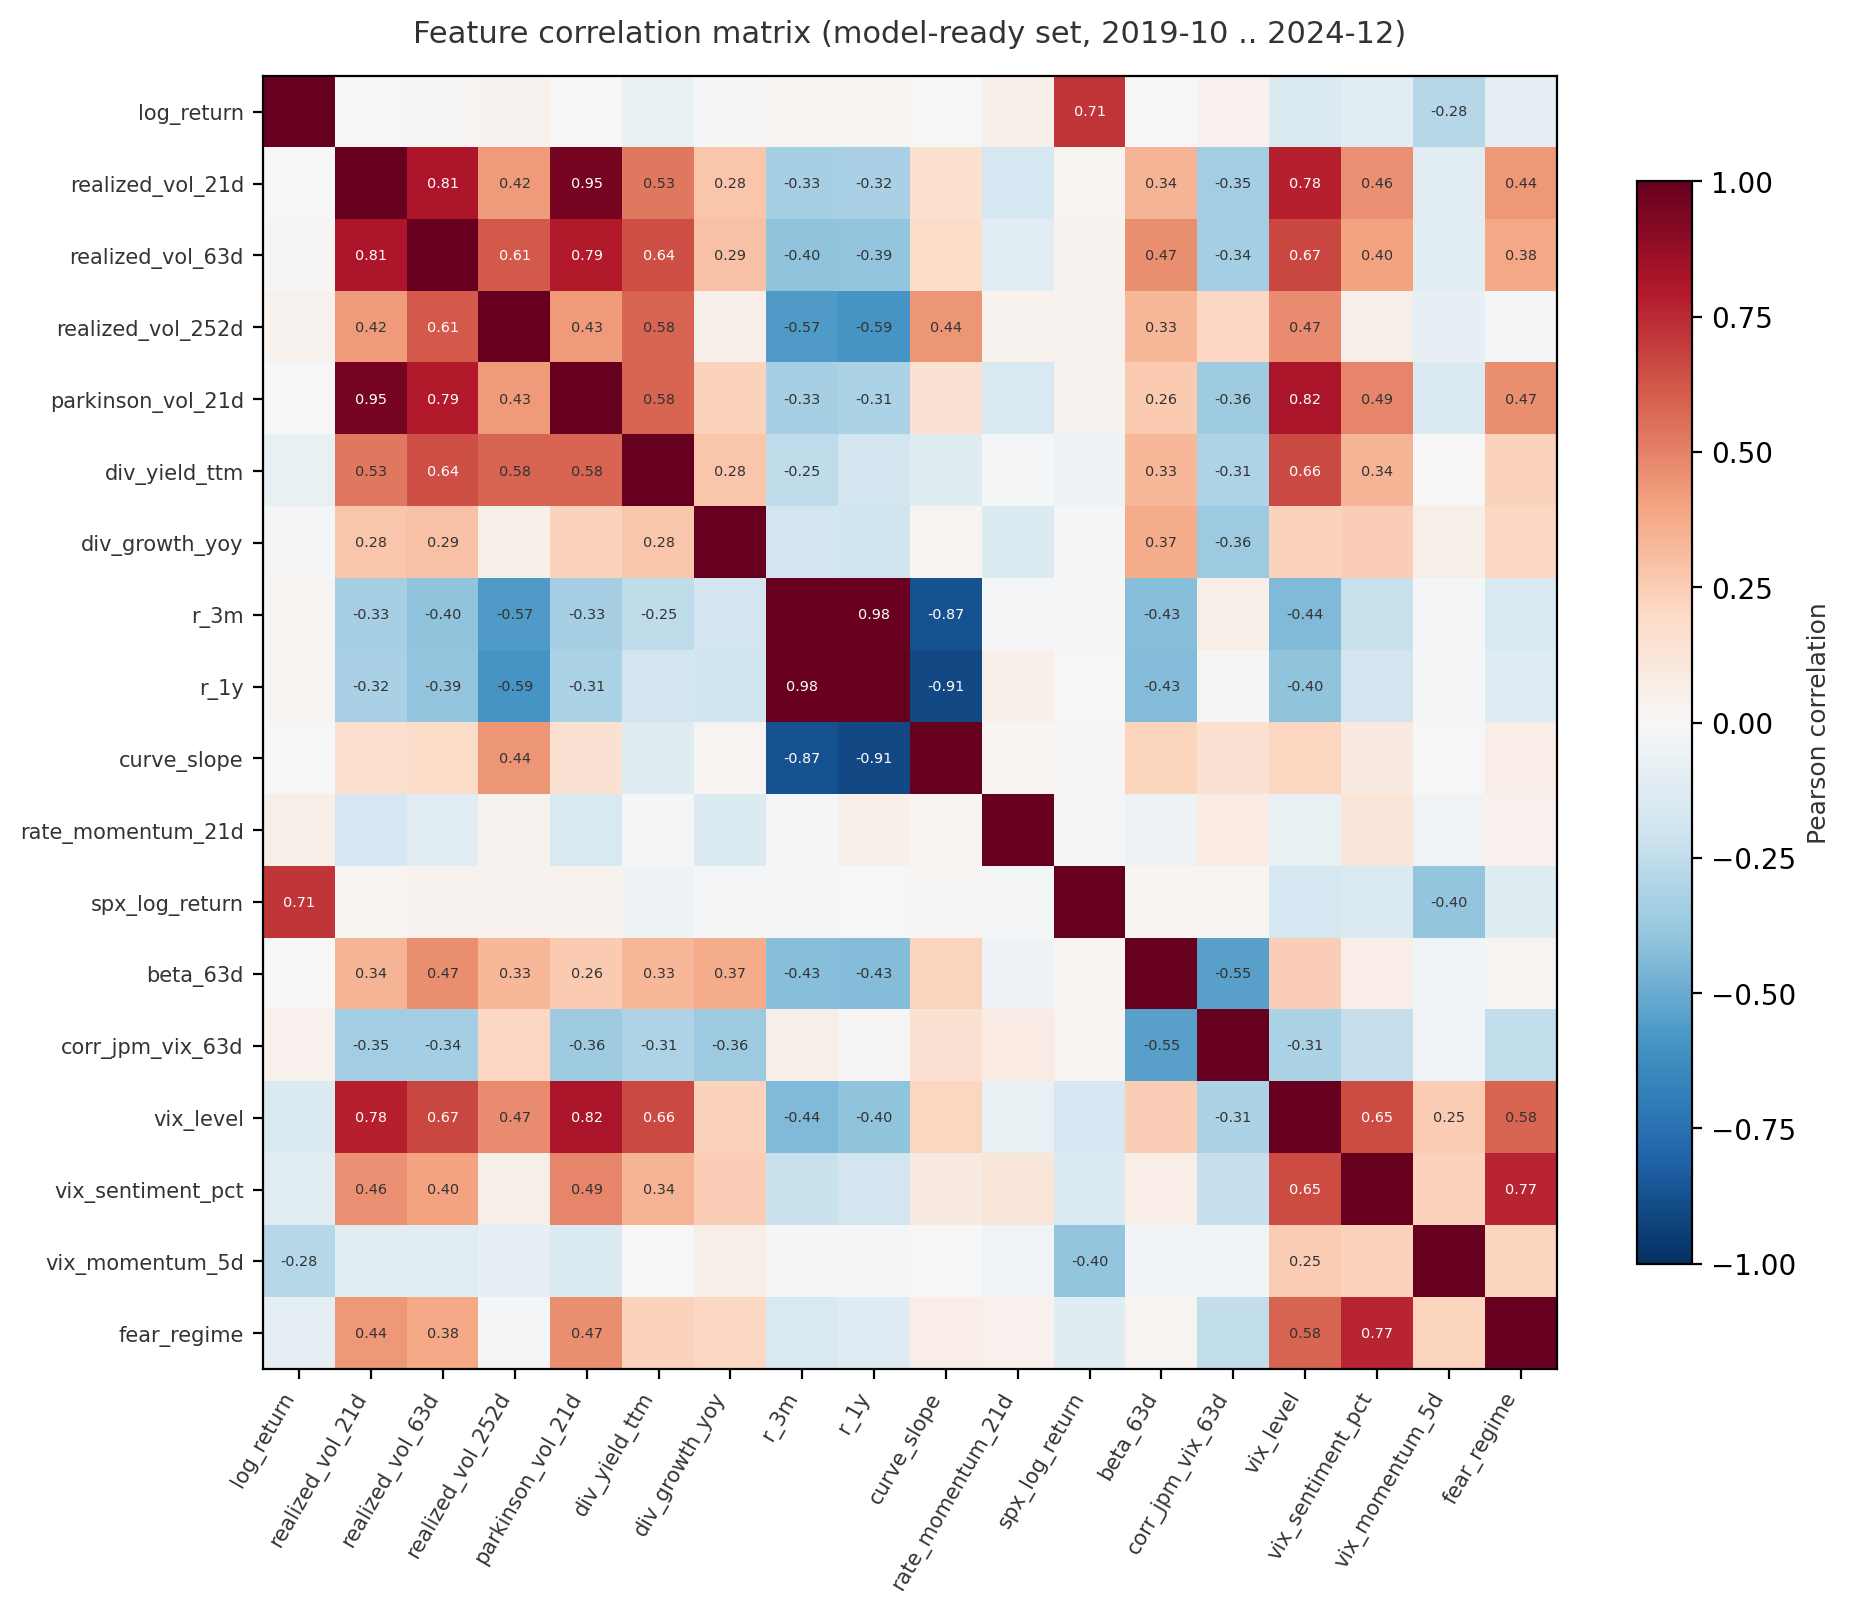
\includegraphics[width=0.88\textwidth]{../../docs/week2/figures/corr_heatmap.png}
\caption{18 特征 Pearson 相关矩阵(仅标注 $|r|\geq 0.25$)}
\end{figure}

结构性发现:(1) \textbf{利率块}:短端两利率相关 $+0.98$,与曲线斜率 $-0.87/-0.91$,对应 2022--23 加息周期的曲线走平/倒挂,建模时线性基线只保留期限匹配的 \texttt{r\_1y};(2) \textbf{波动率块}:五个波动率特征互相关 $0.78$--$0.95$,属预期共线,树模型无碍、线性模型需正则化;(3) VIX 经百分位变换后与已实现波动率的相关从 $\sim$0.8 降至 $\sim$0.45,说明情绪/波动率双角色分离有效。

\subsection{特征重要性}
以\textbf{未来 21 日已实现波动率}(第 5 周 ML 路线 A 的预测目标)为目标变量,随机森林与互信息双口径评估:

\begin{figure}[h!]
\centering
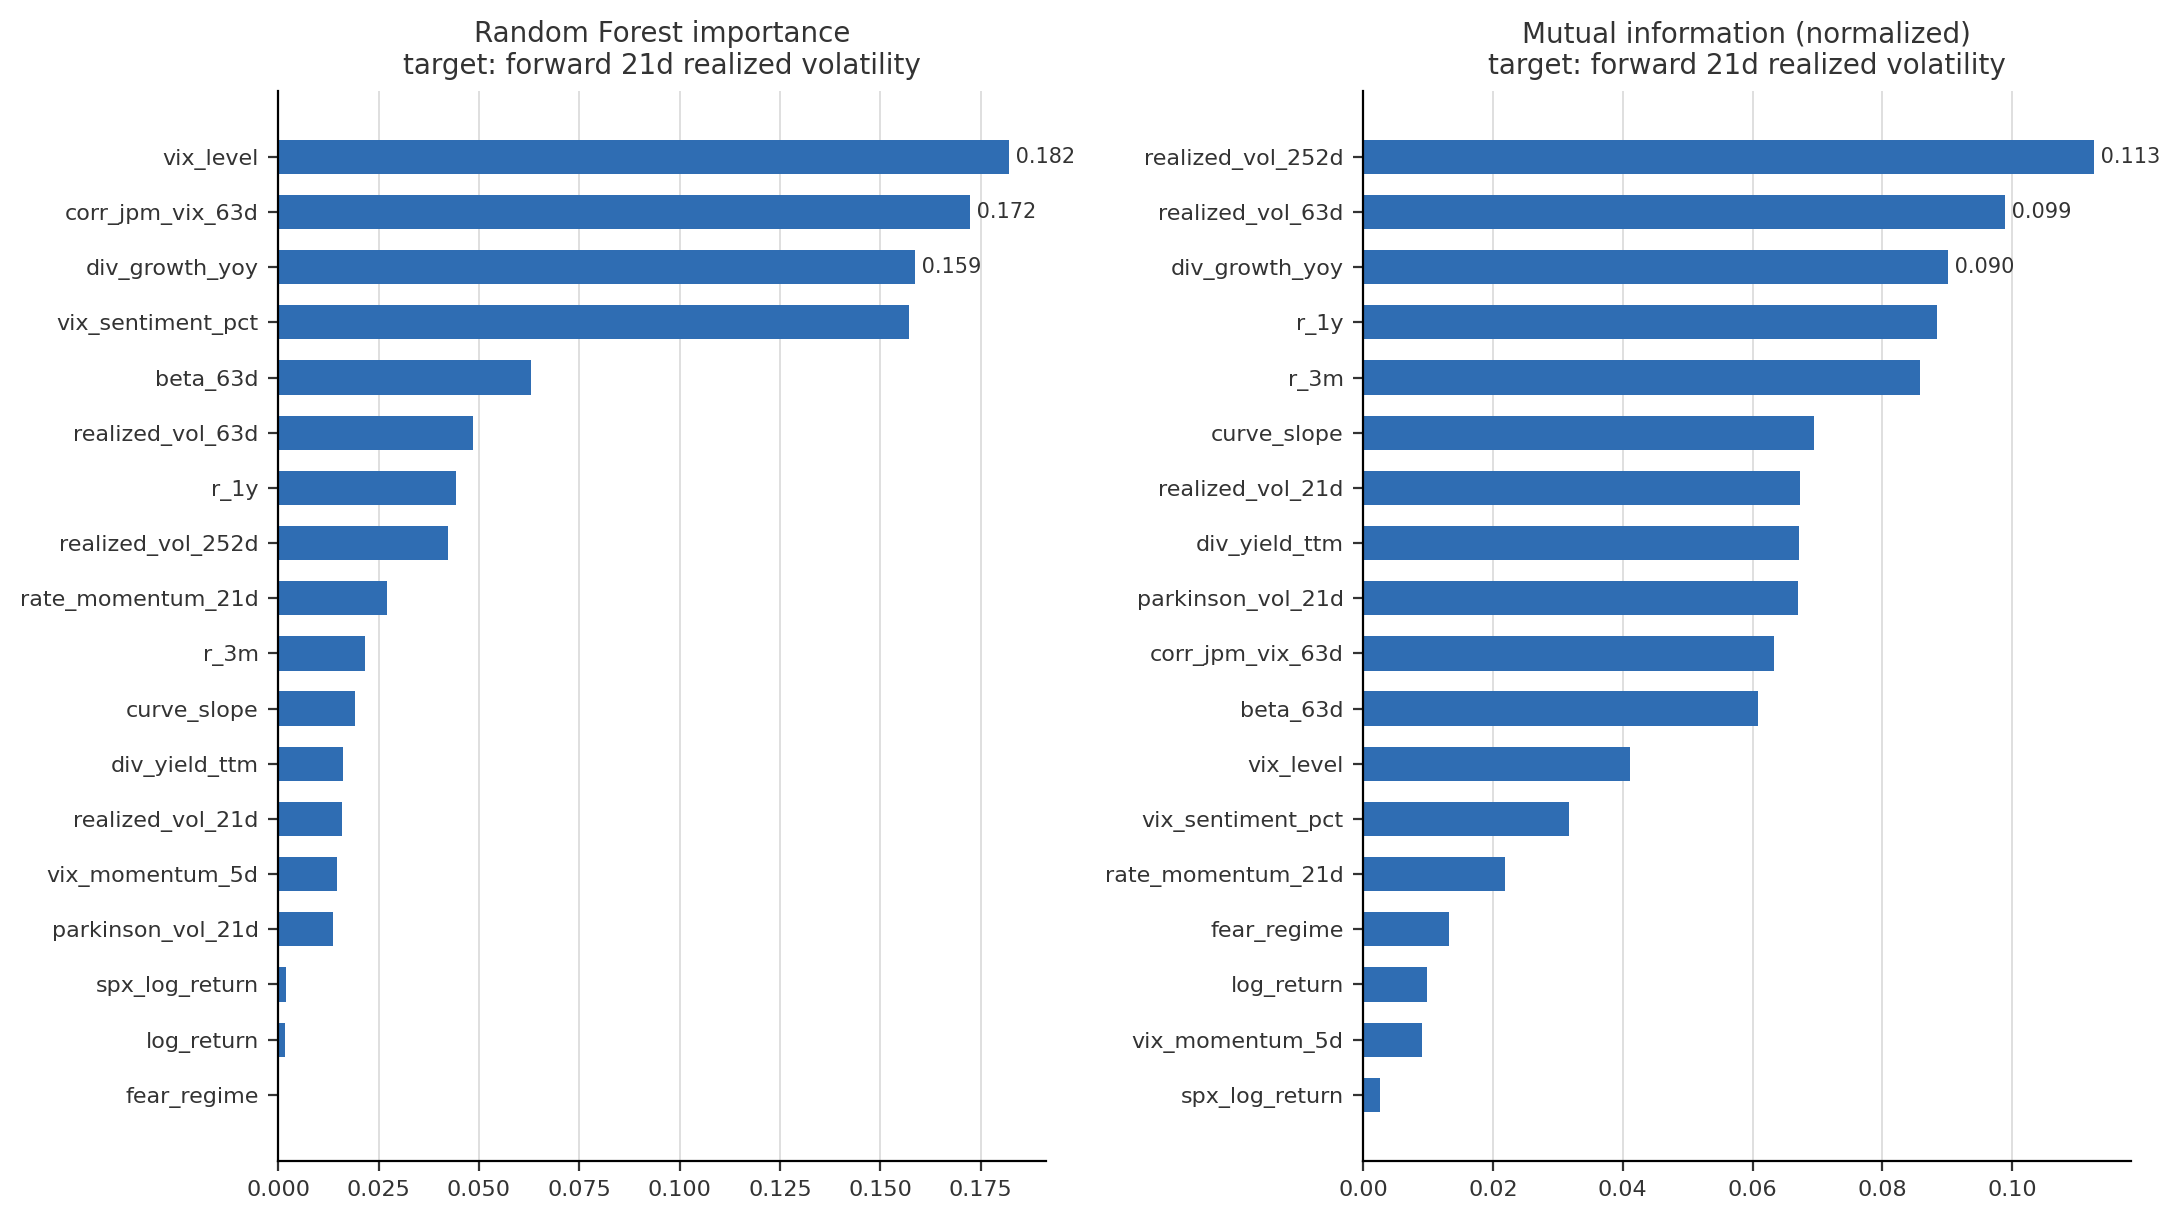
\includegraphics[width=\textwidth]{../../docs/week2/figures/feature_importance.png}
\caption{特征重要性:随机森林(左)、互信息(右)}
\end{figure}

主要结论:(1) RF 口径头部为 \texttt{vix\_level}(0.182)、\texttt{corr\_jpm\_vix\_63d}(0.172)等 \textbf{VIX 系前瞻特征,整体压过回望性的已实现波动率}(与目标的单变量相关亦是 \texttt{vix\_level} 最高,$|r|=0.62$),与方差风险溢价文献一致,为第 5 周``VIX 特征集预测波动率 $\to$ 喂给 BSM''的路线提供数据背书;(2) 互信息口径下长窗口已实现波动率最高(\texttt{realized\_vol\_252d}: 0.113),说明单变量层面波动率长记忆最稳、VIX 的增量主要在多变量交互中体现;(3) \texttt{fear\_regime} 重要性 $\approx 0$(信息被连续版情绪分吸收,相关 $+0.77$),保留仅为可解释性;(4) 本分析为探索性(全样本拟合),第 5--6 周正式训练采用 70/15/15 时序切分防前视偏差。

\section{待对齐事项}
GitHub Actions 生效需在仓库 Settings $\to$ Secrets 配置 \texttt{FRED\_API\_KEY} 与 \texttt{ALPHA\_VANTAGE\_API\_KEY} 两个密钥(本地 \texttt{.env} 不随代码上传)。

\section{下周计划(Week 3:BSM Chooser 模型复现)}
\begin{enumerate}
  \item 实现 Rubinstein (1991) simple chooser 闭式解,以论文 Table 2 参数($S_0=156.7$, $K=150$, $r=0.15\%$, $\sigma=28.2\%$, $q=2.33\%$, $t_1=0.5$, $T_2=1$)算出基准价;
  \item 实现两段 GBM 蒙特卡洛引擎,同时支持``价值最优''与论文``moneyness''两种选择规则,量化后者的价值低估;
  \item 复现论文 Fig.3--6 敏感性曲线($\sigma$、$K$、$r$、$q$),补做论文未竟的 $t_1$ 敏感性分析;
  \item MC 收敛性验证(对照闭式解),为第 4 周基线评估铺路。
\end{enumerate}

\end{document}
